\subsubsection{Model}
%% MIKKEL %%
% Hvordan laves (spawnes) bræt og brikker?
% Hvordan lagres brikker og tiles internt?
Når \texttt{DamModel} instantieres, kører den metoden \texttt{setup}. Denne skaber brættet og brikkerne.\\

\textbf{Bræt:} Felterne der udgør brættet gemmes i et \texttt{Tile}$[\, \, \,][\,\,\,]$ \texttt{board}. Klassen \texttt{Tile} indeholder fields for dens koordinater på brættet, samt om det er et lyst eller mørk felt og om feltet er optaget. Her er også metoderne \texttt{getOccupied} og \texttt{setOccupied}, der vedrører om et felt er optaget. Brættet sættes op ved metoden \texttt{setupBoard} i klassen \texttt{DamModel}. \texttt{setupBoard\texttt} laver felter med skiftende farve, og tilføjer dem til \texttt{board}.

\begin{figure}[H]
\centering
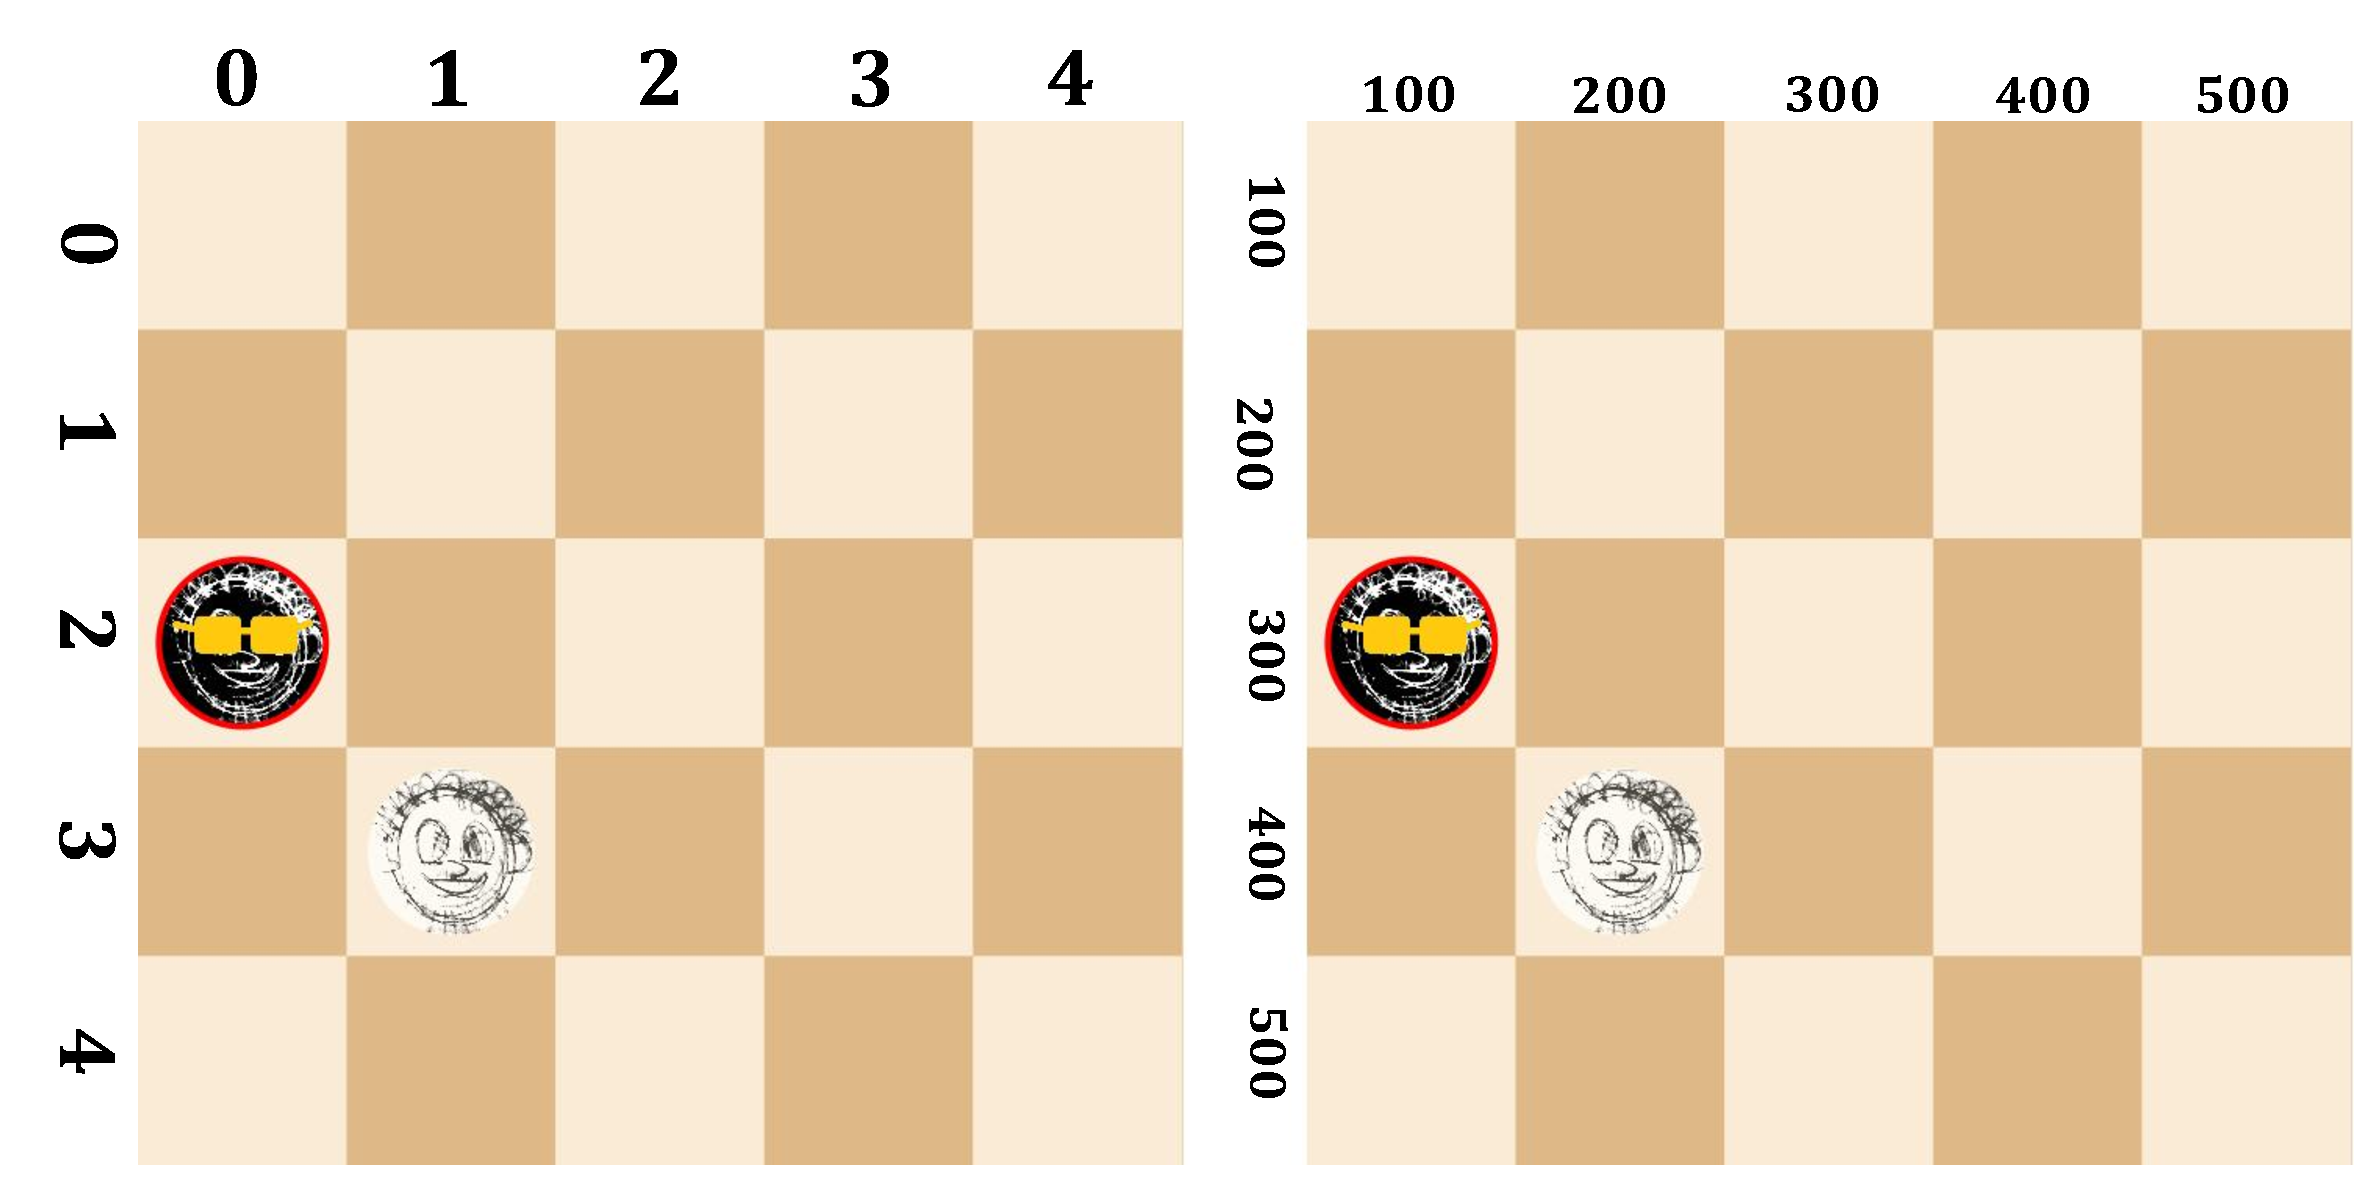
\includegraphics[width = 0.8 \textwidth]{Figurer/modelCoordViewCoord.pdf}
\caption{Model koordinater sammenlignet med View koordinater. Bemærk, at View koordinater varierer fra skærm til skærm, og koordinaterne her svarer blot til én computers koordinater.}
\label{fig:modelCoordViewCoord}
\end{figure}

% Mikkel
\textbf{Brikker:} Brikkerne lagres i en \texttt{ArrayList<Piece> pieces}.

Klassen \texttt{Piece} indeholder fields for sine koordinater på brættet, koordinater på skærmen, hvilken spiller den tilhører, dens farve og størrelse (radius). I \texttt{Piece} findes også metoden \texttt{move}, der håndterer flytning af brikken. Brikkerne sættes op ved metoden \texttt{setupPieces}. \texttt{setupPieces} kører metoden \texttt{placePiece}, og skaber to \texttt{pieces}, i hvert deres hjørne af brættet, og sætter deres hold. Deres positioner bliver sat ud fra \texttt{tileAmount}, så de står i hjørnerne uafhængigt af størrelsen af brættet. Metoden \texttt{placePiece} tager et objekt af typen \texttt{Piece}, og tilføjer det til \texttt{ArrayListen pieces}. Derudover tilføjer \texttt{placePiece} brikken til layoutet, og gør brikkens felt optaget.
